\section{Assemblies of DC1 and Tsth20}

Prior to assembly of DC1 and Tsth20 sequences, the tool FastQC was
used to evaluate the quality of the Illumina sequences provided for
this project. After trimming the Illumina sequences for low quality
reads, one FAIL flag was raised for both samples. This was the
per-sequence GC content flag, indicating that the GC content of
high-quality did not meet expectations. Plots of GC content for the
trimmed R1 sequences of both DC1 and Tsth20 are shown in
figure~\ref{fig:fastqc-lowgc}. In these plots, there is a considerable
increase in the number of sequences with GC content between 2 and 30\%,
which is important to note for later results and discussion.

\begin{figure}
  \centering
  \begin{subfigure}{0.8\textwidth}
    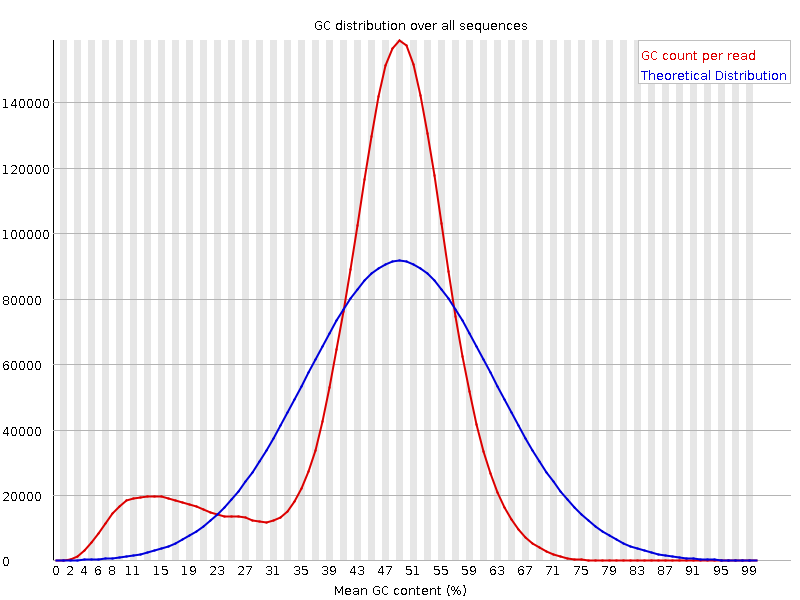
\includegraphics[width=\textwidth]{/Users/cbe453/Desktop/masters/masters/masters/working-thesis/figures/dc1-low-gc-fastqc.png}
    \caption{DC1}
    \label{fig:dc1fastqc}
  \end{subfigure}
  \\
  \begin{subfigure}{0.8\textwidth}
  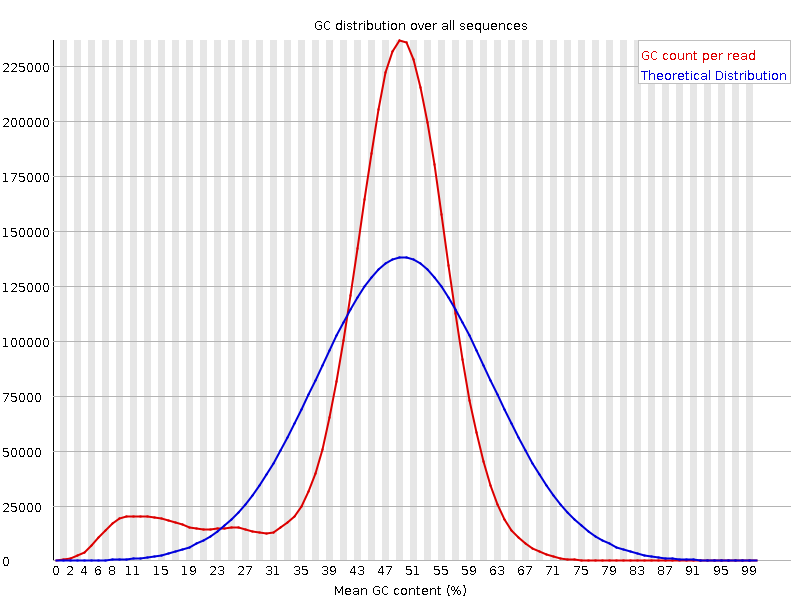
\includegraphics[width=\textwidth]{/Users/cbe453/Desktop/masters/masters/masters/working-thesis/figures/tsth20-low-gc-fastqc.png}
    \caption{Tsth20}
    \label{fig:tsth20fastqc}
  \end{subfigure}
  \caption{Plots showing the distribution of GC content in Illumina
    sequences.}
  \label{fig:fastqc-lowgc}
\end{figure}

A sliding window analysis was also performed on all final assemblies
in order to identify regions of anomalous GC content. The results of
this analysis are shown in figure~\ref{fig:assembly-gc}. Of the
included assemblies, anomalous GC content was identified in DC1,
Tsth20, \textit{T. reesei} and \textit{T. harzianum}, with
\textit{T. virens} showing no anomalous GC content. In addition to the
confirmation of anomalous GC content, it appears that the distribution
of GC content in \textit{T. reesei} differs from the other assemblies.

\begin{figure}
  \begin{center}
    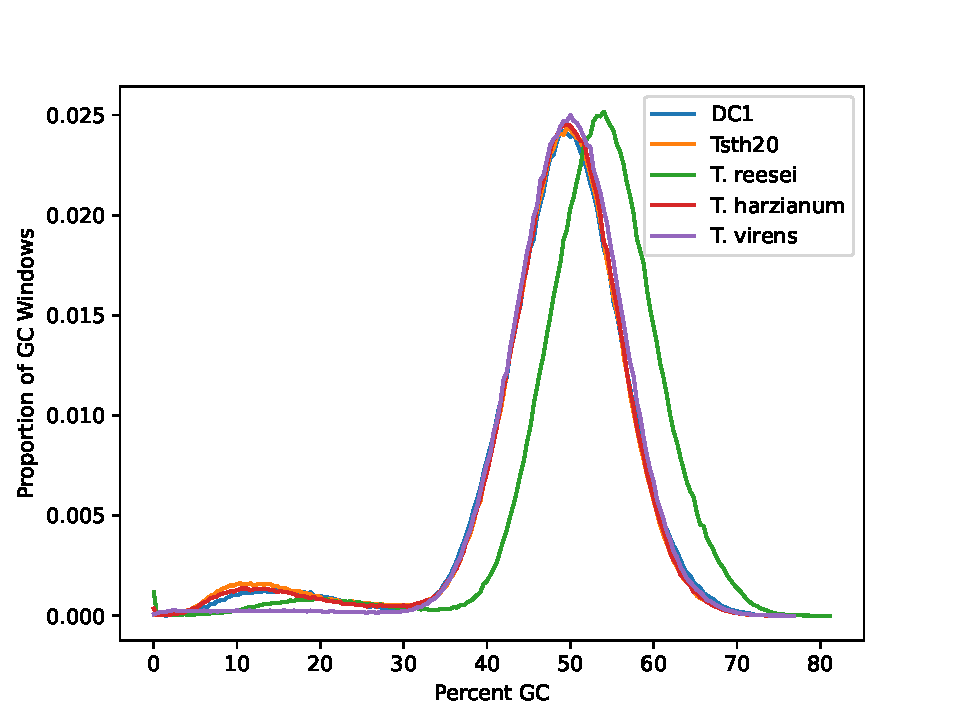
\includegraphics[width=0.8\textwidth]{figures/gc-plot.pdf}
  \end{center}
  \caption{Plots showing the frequency of GC values calculated from
    sliding windows for each assembly.}
  \label{fig:assembly-gc}
\end{figure}

For other general assembly metrics, the QUAST tool was used. Results
from QUAST are shown in figure~\ref{table:assemblies}, from which we can
make several observations. The most obvious observation to start with
is total contig counts for each assembly. For DC1 and Tsth20, the
total contig counts are an order of magnitude smaller when compared to
the other NCBI RefSeq assemblies, inidicating highly contiguous
assemblies from nextDenovo and nextPolish. This is likely due to the
use of long-read sequencing used in the assemblies of DC1 and
Tsth20. The total assembly lengths are similar, hovering around the
38-42Mb range, except in the case of \textit{T. reesei}, which is
known to have a significantly smaller genome length (ref) at roughly
33Mb. The largest contig size for each assembly vary greatly. DC1 and
Tsth20 have the largest contigs of all assemblies being considered,
which is again likely due to the inclusion of long-read sequencing
data in the assembly process. The N50 values for all assemblies are
above 1Mb, with DC1 and Tsth20 N50s being at minimum three times
larger than others assemblies.


\begin{table}
  \begin{center}
    \begin{tabular}{|c|c|c|c|c|c|c|}
      \hline
      Strain & Total Contigs & Total Length & Largest Contig & GC\% & N50 & L50 \\ \hline
      DC1 & 8 & 38.6 Mb & 11.49 Mb & 47.97 & 5.69 Mb & 3 \\ \hline
      Tsth20 & 7 & 41.58 Mb & 8.02 Mb & 47.33 & 6.52 Mb & 3 \\ \hline
      \textit{T. harzianum} & 532 & 40.98 Mb & 4.08 Mb & 47.61 & 2.41 Mb & 7 \\ \hline
      \textit{T. virens} & 93 & 39.02 Mb & 3.45 Mb & 49.25 & 1.83 Mb & 8 \\ \hline
      \textit{T. reesei} & 77 & 33.39 Mb & 3.75 Mb & 52.82 & 1.21 Mb & 9 \\ \hline
    \end{tabular}
  \end{center}
  \caption{General assembly metrics produced by QUAST (a
    genome quality assement tool).}
  \label{table:assemblies}
\end{table}


